\documentclass[hyperref={pdfpagelabels=false}]{beamer}
\let\Tiny=\tiny
\usepackage{amsmath,amsfonts,amsthm,amssymb}
\usepackage{subfigure}
\usepackage{booktabs}
\usepackage{color}
%\usepackage{movie15}
\usepackage{eulervm}
\usepackage{palatino}
%\usepackage{concrete}
%\usepackage{charter}
%\usepackage{courier}
% \usetheme{Warsaw}
% \usefonttheme{serif}
\usetheme{Singapore}

\title{Master's Presentation}
\subtitle{Robot Traffic School}
\author{Thomas Denewiler}
%\institute{UCSD/SPAWAR}
%\institute{SPAWAR}
\institute{UCSD}
\date{January 31, 2011}

\begin{document}

% Define new variables.
\def\argmin{\mathop{\arg\,\min}\limits}
\def\argmax{\mathop{\arg\,\max}\limits}

\begin{frame}
\titlepage
\end{frame}

\begin{frame}{Outline}
\begin{itemize}
\item Problems with original robot navigation.
\item Kalman filter implementation.
\item Kalman filter bugs.
\item Training the noise models.
\item Kalman filter improvements.
\item Model based controller.
\item Practical considerations for gains.
\item Controller improvements.
\end{itemize}
\end{frame}

\begin{frame}{Motivation}
\begin{itemize}
\item Robots sometimes drive like they are drunk.
\item Errors are a combination of estimation and control.
\end{itemize}
\begin{figure}
    \centering
    \mbox{
        \subfigure{
            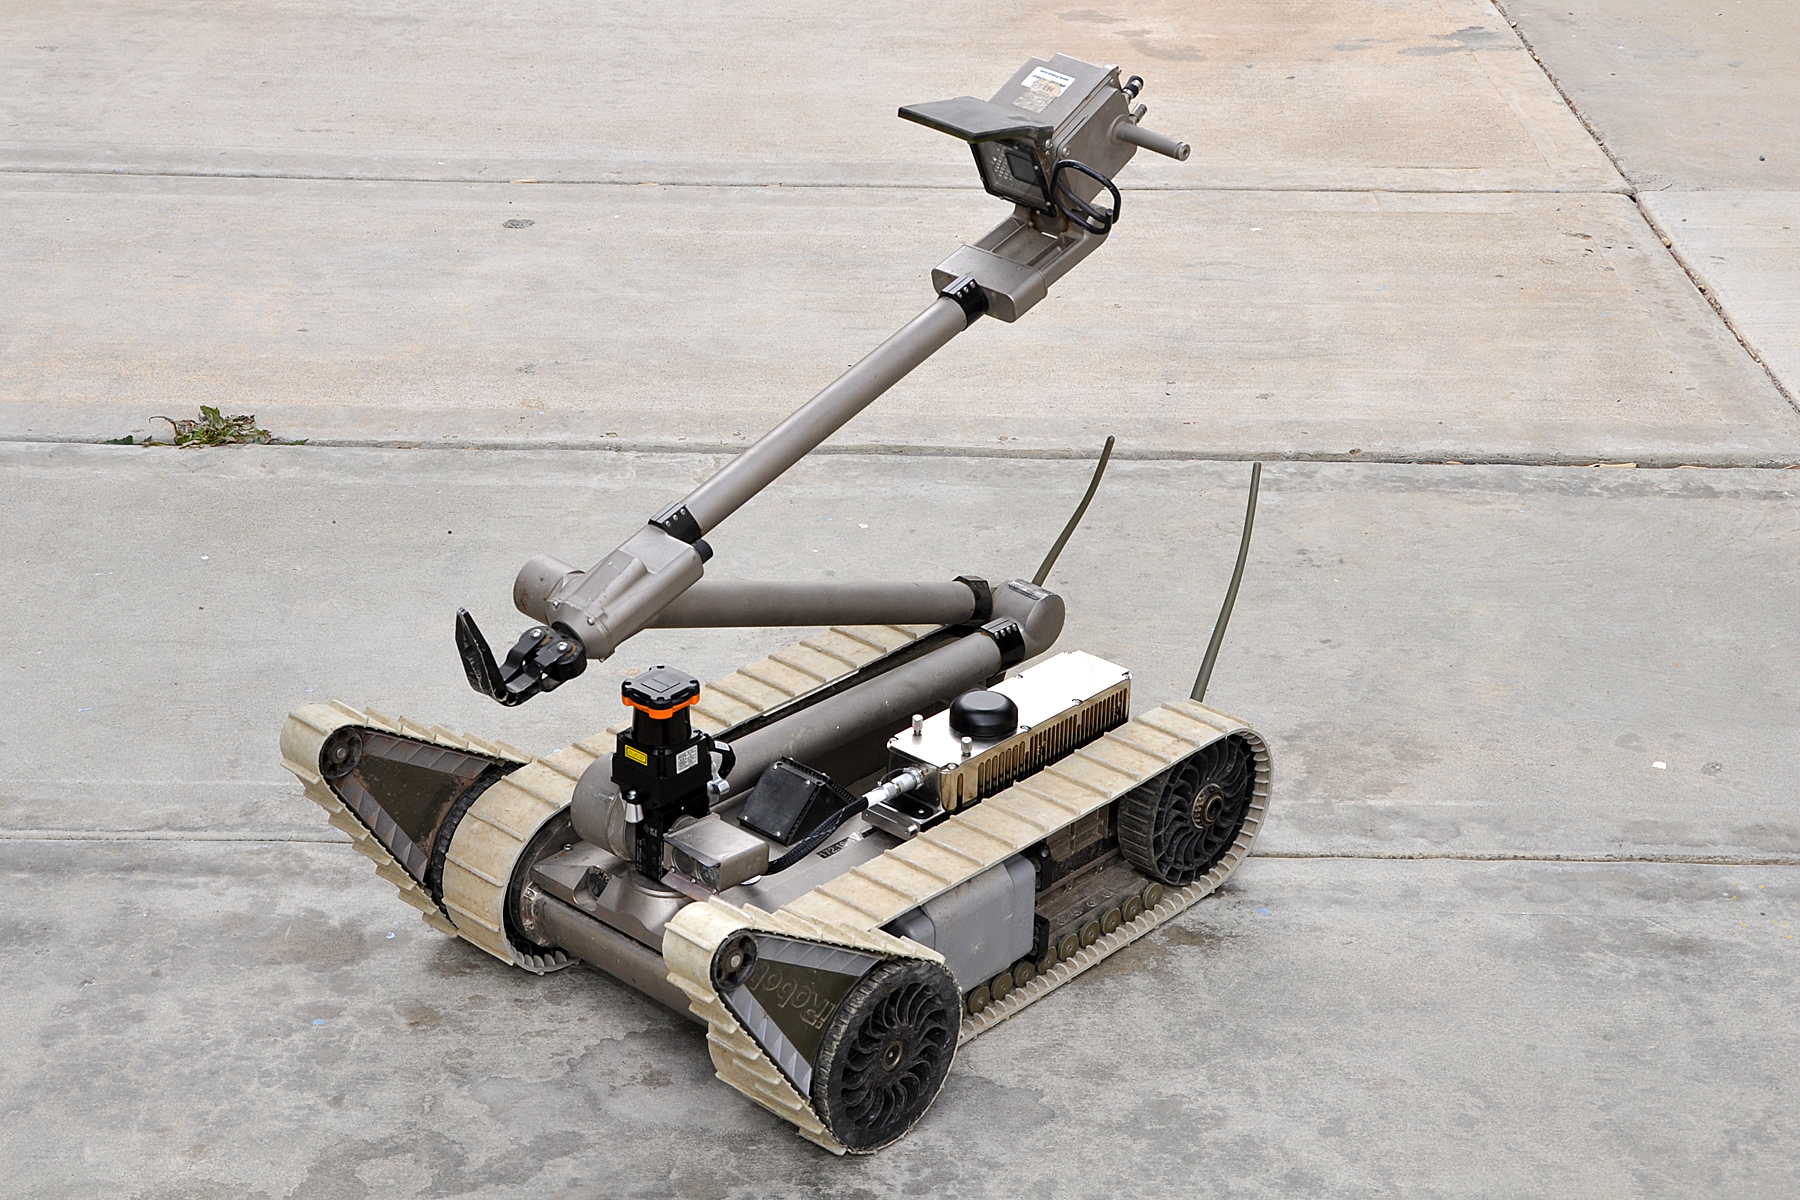
\includegraphics[height=.3\textheight]{images/packbotRetrotraverse}
            \quad
            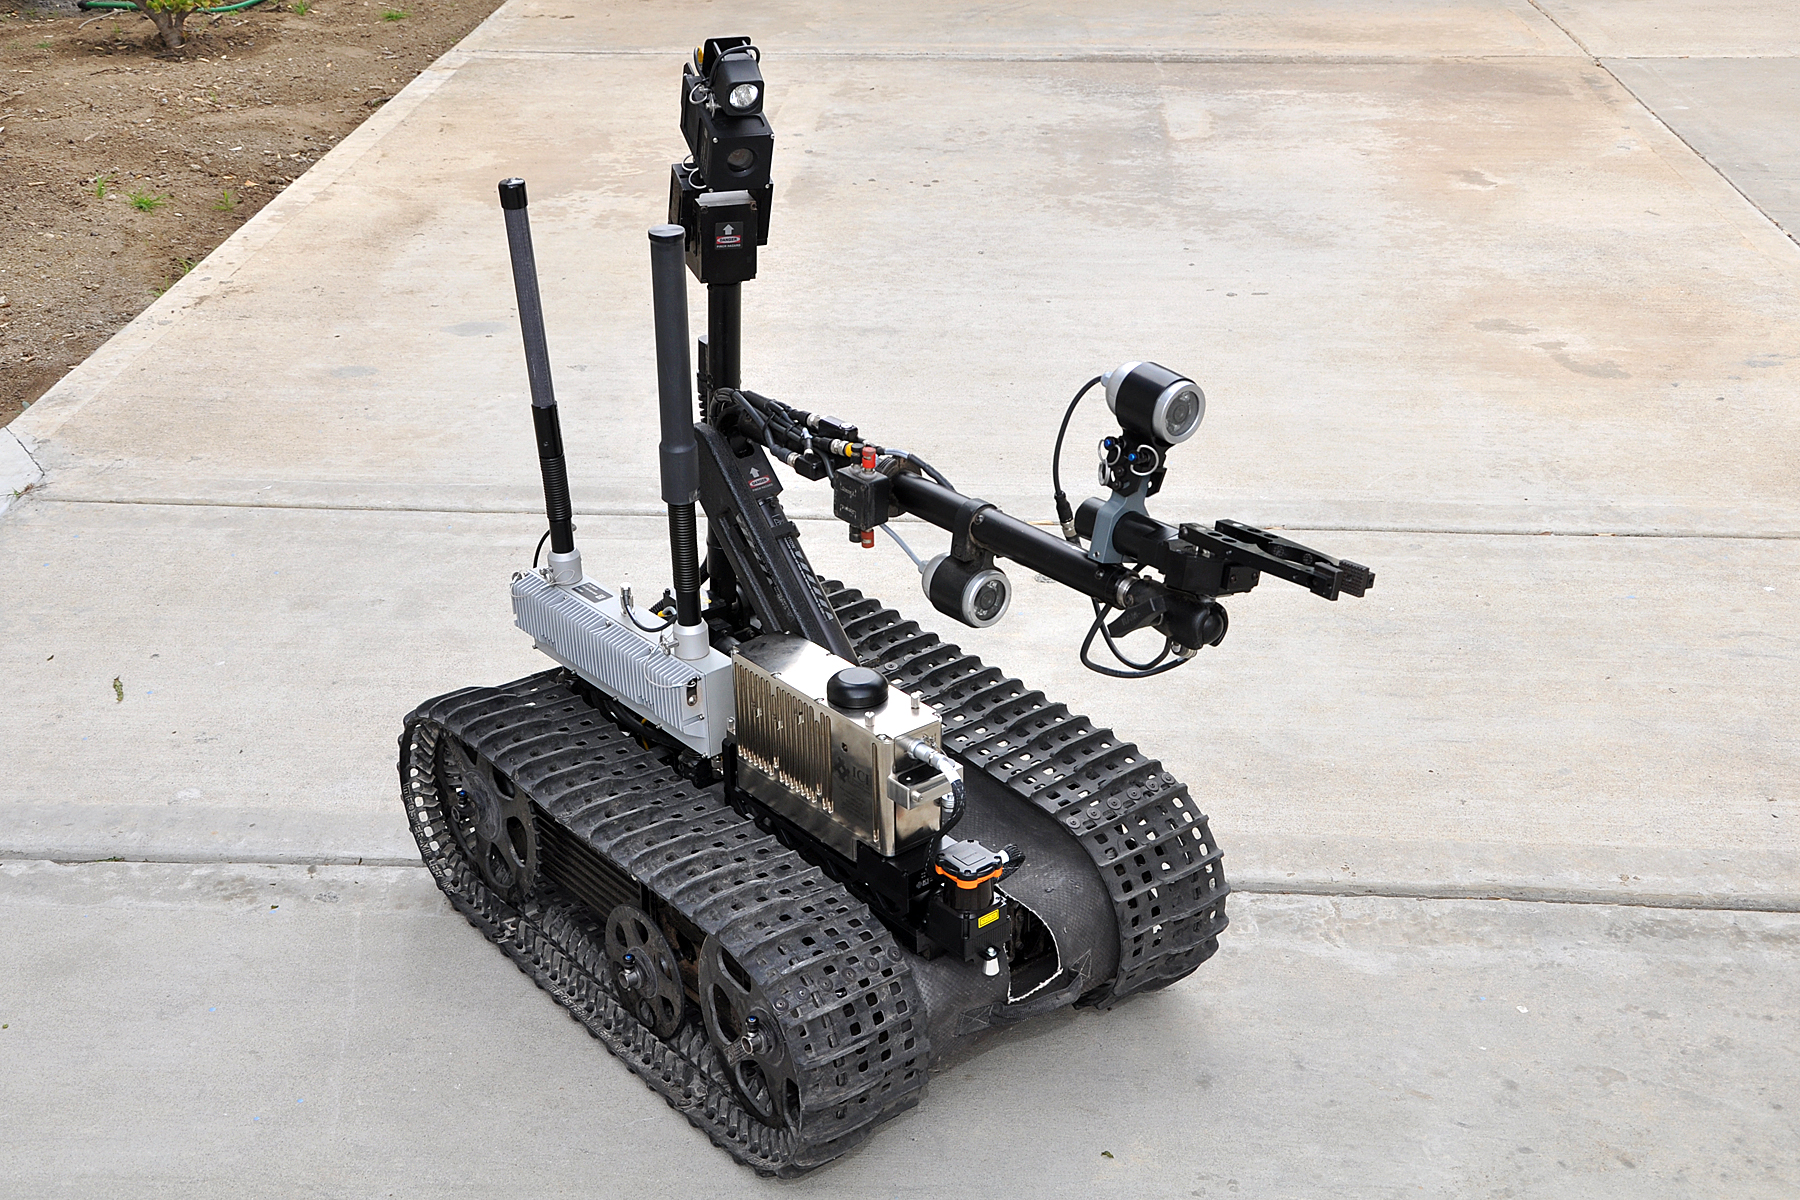
\includegraphics[height=.3\textheight]{images/talonRetrotraverse}
        } % end subfigure
    } % end mbox
\end{figure}
\begin{figure}
    \centering
    \mbox{
        \subfigure{
            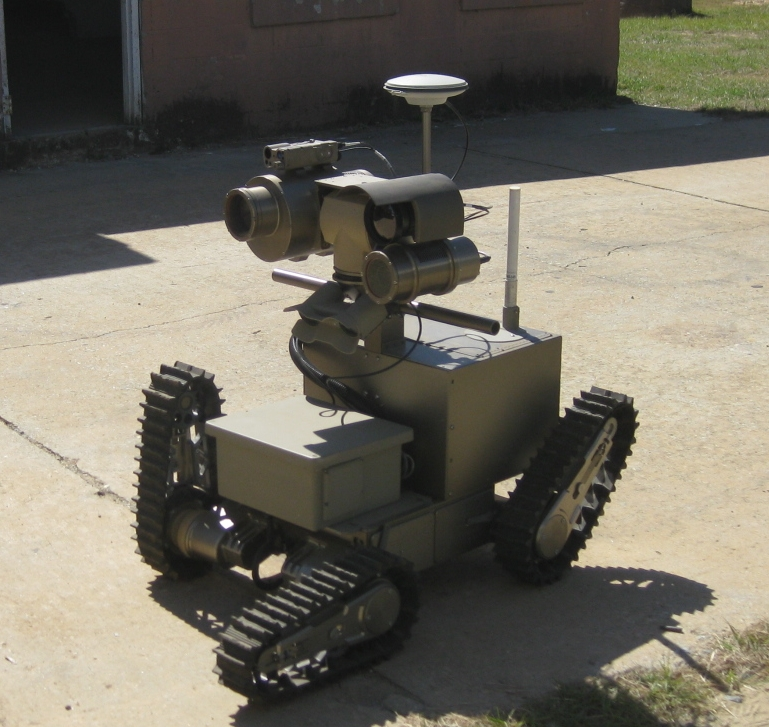
\includegraphics[height=.3\textheight]{images/chaos}
            \quad
            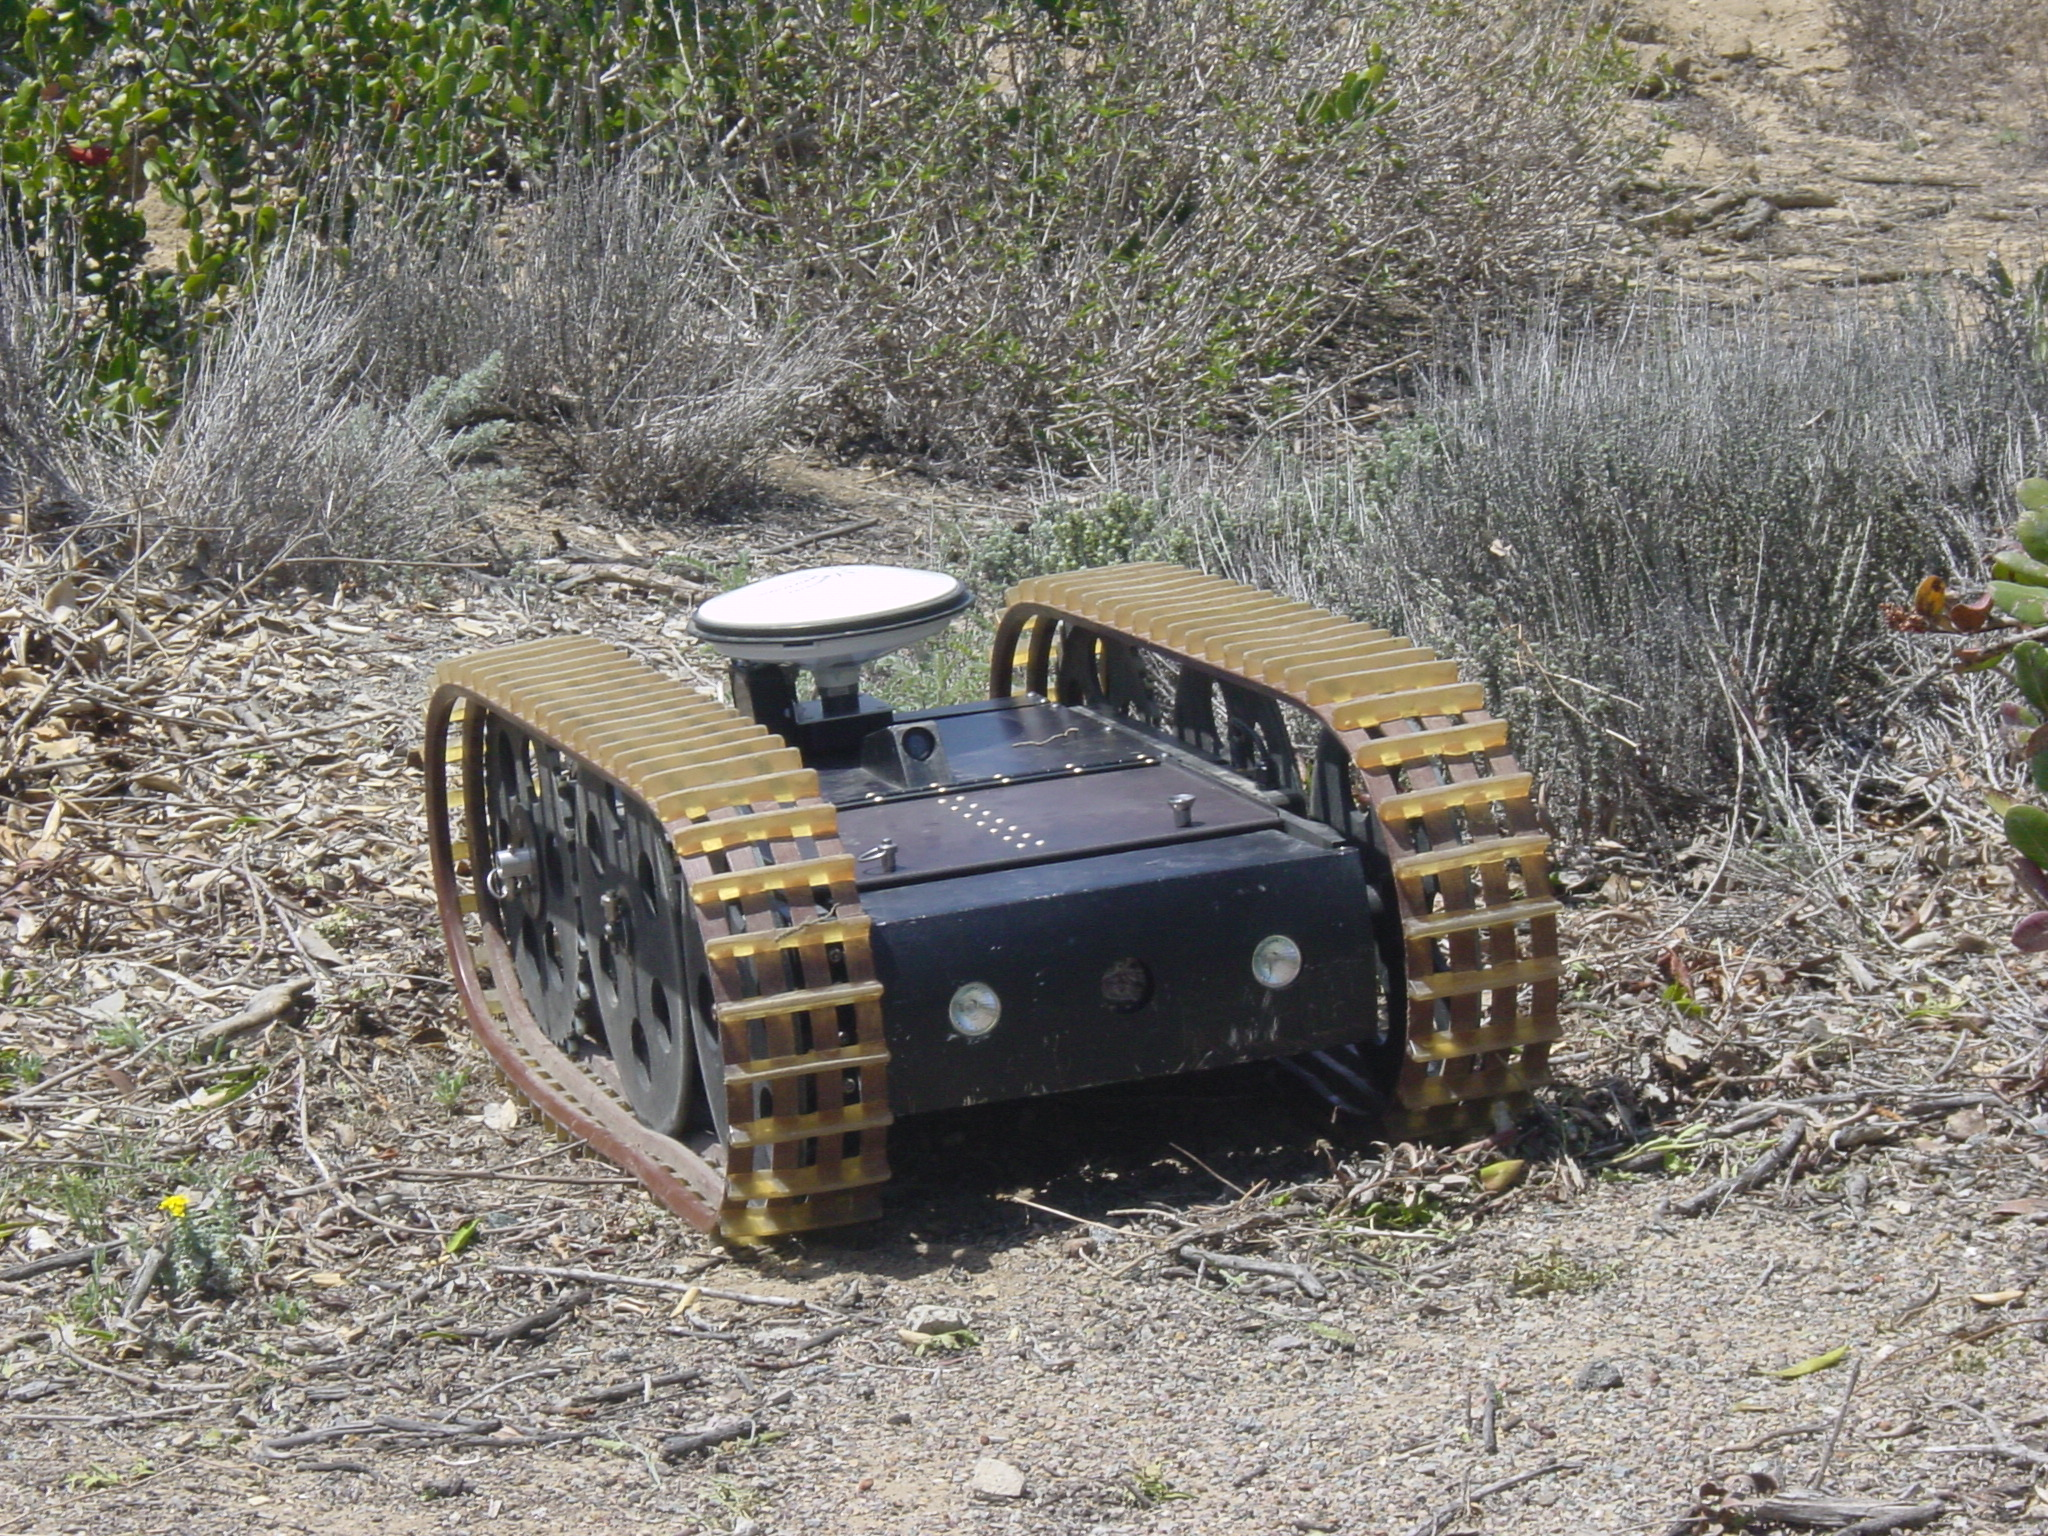
\includegraphics[height=.3\textheight]{images/urbotWithGps}
        } % end subfigure
    } % end mbox
\end{figure}
\end{frame}

\begin{frame}{Drunk Robots}
% Put in a movie of Packbot with PID controller here.
\begin{itemize}
\item PID Packbot movie here.
\end{itemize}
\end{frame}

\begin{frame}{Robot States}
\begin{itemize}
\item The states are $x$, $y$, $z$ positions, $\theta$, $\phi$, $\psi$ Euler angles (pitch, roll, yaw) and $V$, $\omega$ velocities (linear, angular).
\item Body frame coordinate system.
\item A coordinate frame transformation is needed to convert to world coordinate system.
\end{itemize}
\begin{figure}[ht!]
    \centering
    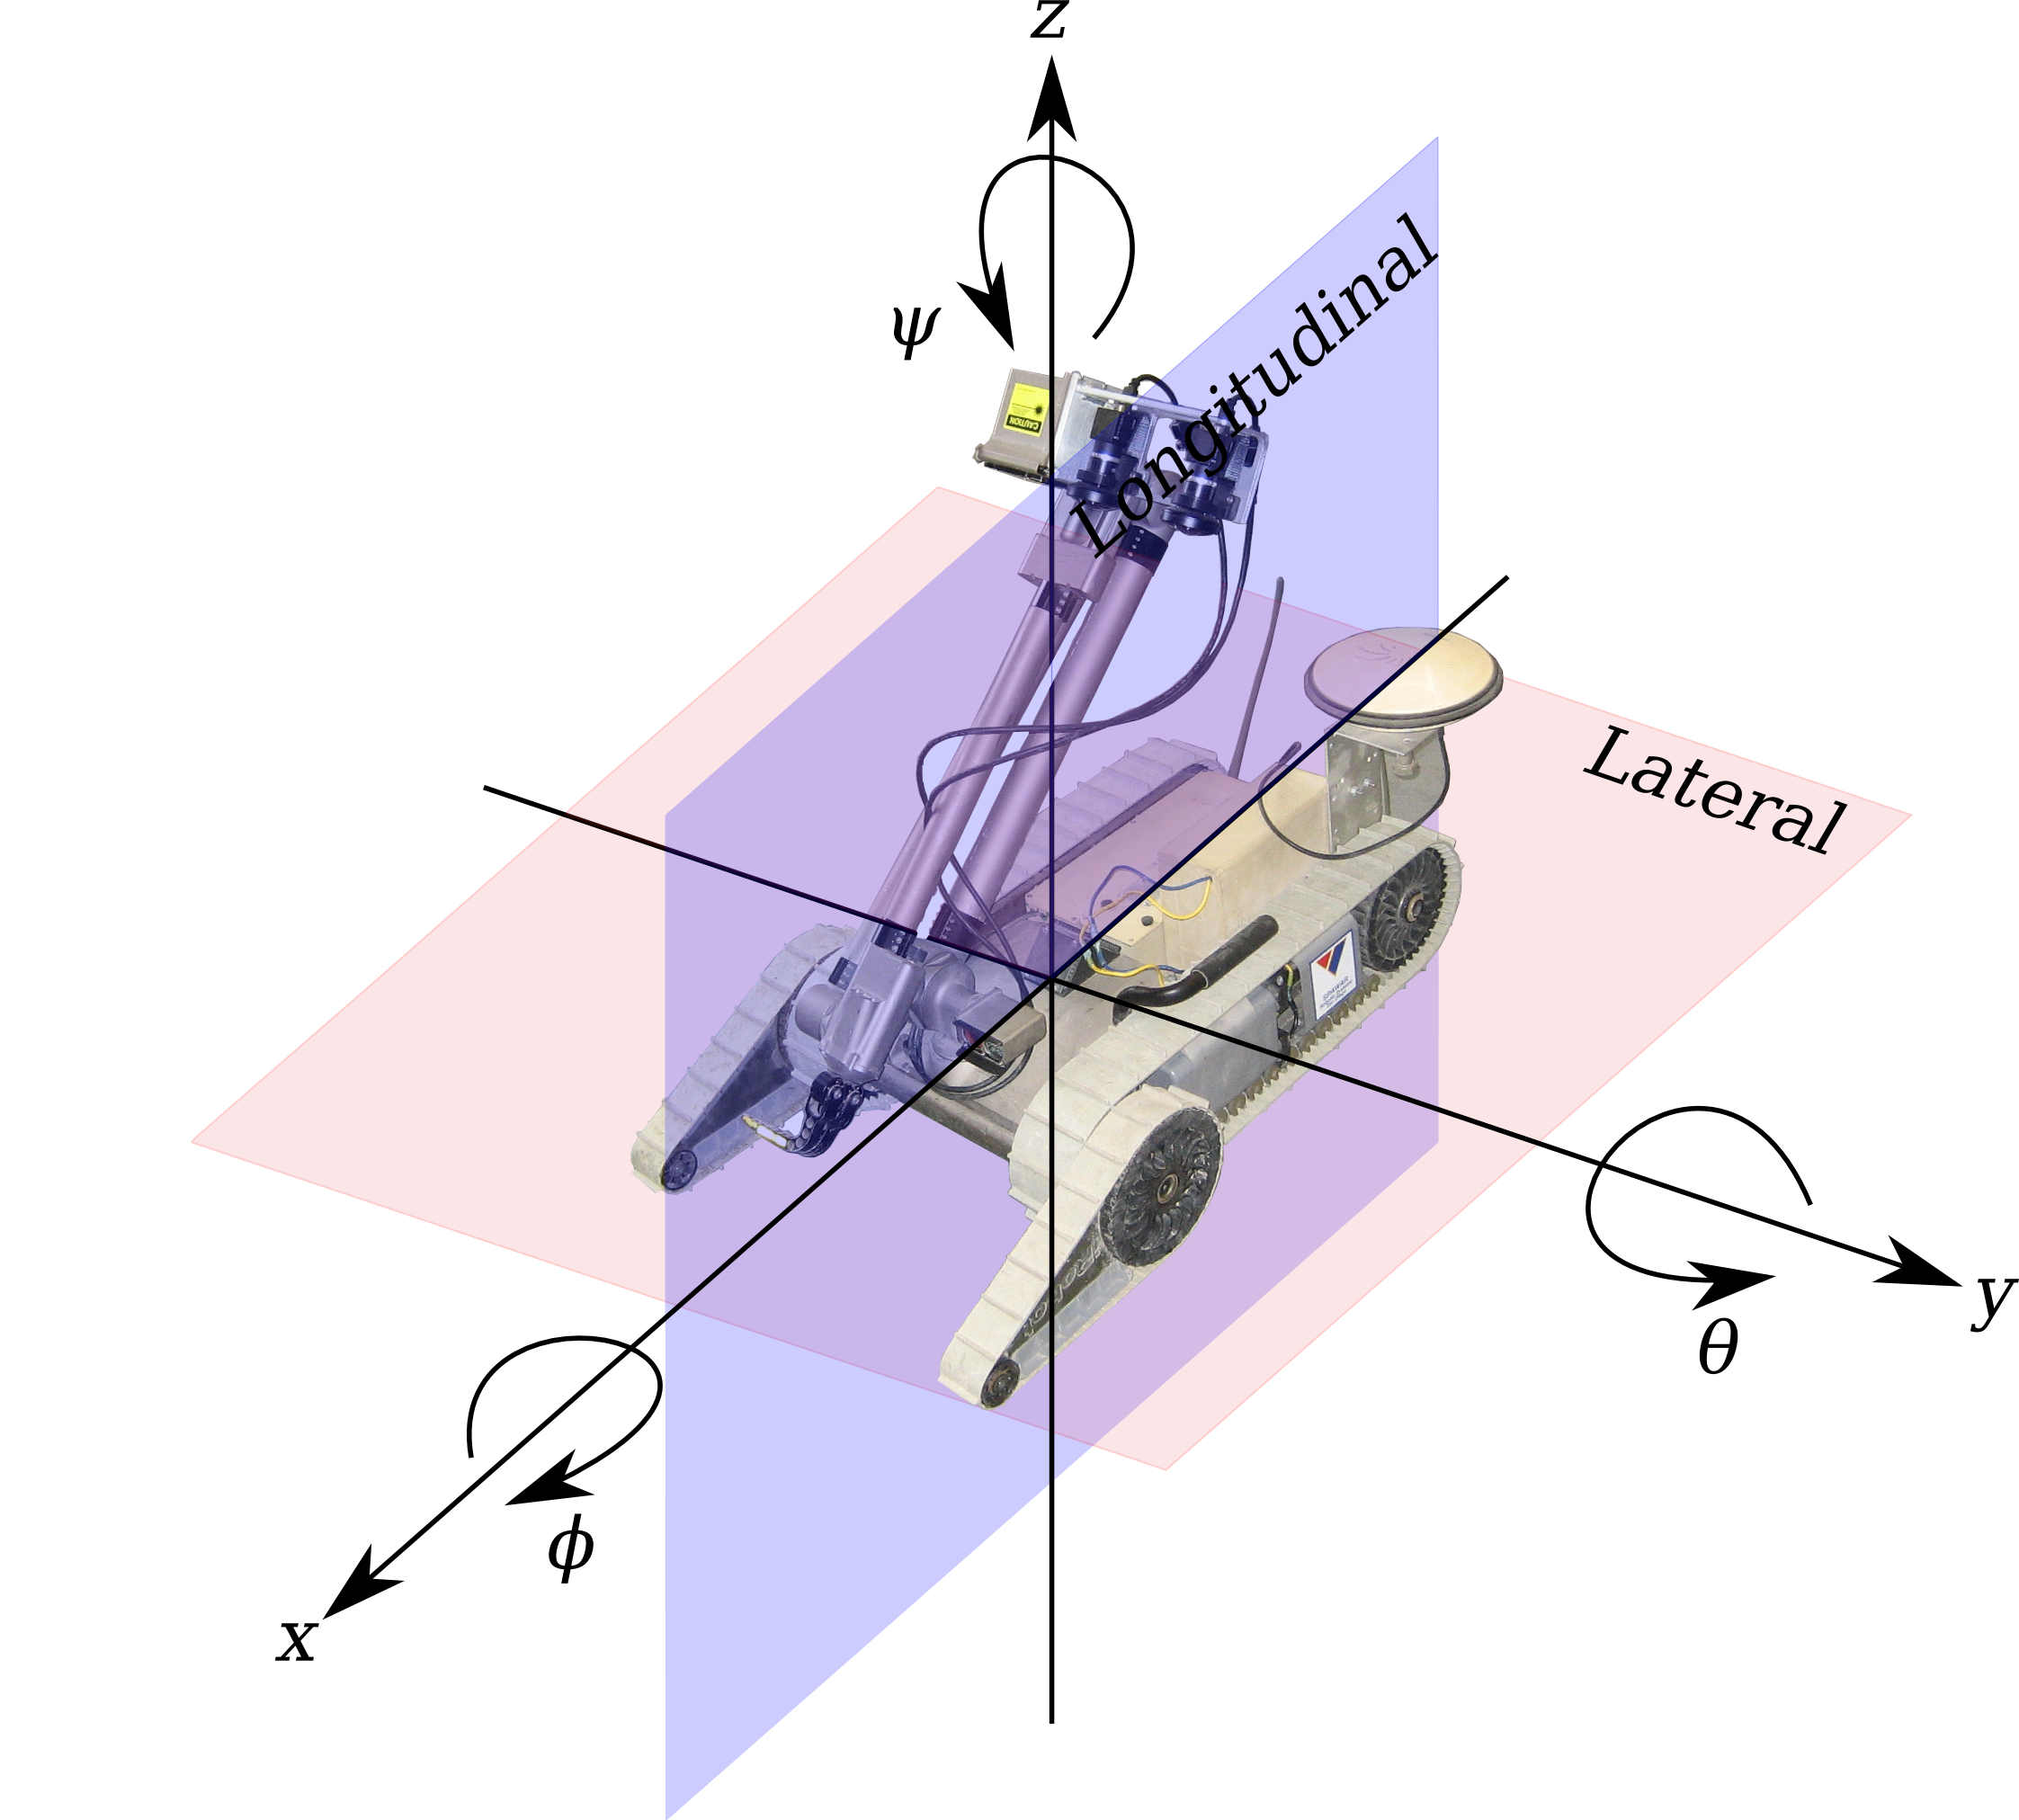
\includegraphics[width=.5\textwidth]{images/packbotaxes}
\end{figure}
\end{frame}

\begin{frame}{System Model}
\begin{itemize}
\item A nonlinear model based on the robot kinematics.
\item In body frame coordinate system.
\item $\dot{x} = f(x)$
\end{itemize}
\begin{align*}
\frac{d}{dt}\left[\begin{array}{c}
x \\ y \\ z \\ V \\ \theta \\ \phi \\ \psi \\ \omega
\end{array}\right] =
\left[\begin{array}{c}
V\cos\psi\cos\theta \\
V\sin\psi\cos\theta \\
-V\sin\theta \\
0 \\
-\omega\sin\phi \\
\omega\tan\theta\cos\phi \\
\omega\cos\phi/\cos\theta \\
0
\end{array}\right]
\end{align*}
\end{frame}

\begin{frame}{Continuous Time System Model}
\begin{itemize}
\item Jacobian of nonlinear kinematic model.
\end{itemize}
{\tiny
\begin{align*}
\frac{d}{dt}\left[\begin{array}{c}
\Delta x \\ \Delta y \\ \Delta z \\ \Delta V \\ \Delta \theta \\ \Delta \phi \\ \Delta \psi \\ \Delta \omega
\end{array}\right] =
\underbrace{\left[\begin{array}{c c c c c c c c}
0 & 0 & 0 & c\psi c\theta & -V c\psi s\theta               & 0                     & -V s\psi c\theta & 0 \\
0 & 0 & 0 & s\psi c\theta & -V s\psi s\theta               & 0                     & V c\psi c\theta  & 0 \\
0 & 0 & 0 & -s\theta      & -V c\theta                     & 0                     & 0                & 0 \\
0 & 0 & 0 & 0             & 0                              & 0                     & 0                & 0 \\
0 & 0 & 0 & 0             & 0                              & -\omega c\phi         & 0                & -s\phi \\
0 & 0 & 0 & 0             & \omega c\phi/c^2\theta         & \omega t\theta s\phi  & 0                & t\theta c\phi \\
0 & 0 & 0 & 0             & \omega s\theta c\phi/c^2\theta & -\omega s\phi/c\theta & 0                & c\phi/c\theta \\
0 & 0 & 0 & 0             & 0                              & 0                     & 0                & 0
\end{array}\right]}_{F}
\left[\begin{array}{c}
\Delta x \\ \Delta y \\ \Delta z \\ \Delta V \\ \Delta \theta \\ \Delta \phi \\ \Delta \psi \\ \Delta \omega
\end{array}\right]
\end{align*}
}
\end{frame}

\begin{frame}{Discrete Time System Model}
\begin{itemize}
\item The system model is simplified by invoking the low dynamics assumption and the principal motion assumption.
\item Moving from continuous time to discrete time is done by $\Phi_k = I + F\Delta_T$.
\item Positions depend on previous state and linear velocity, orientation on previous state and angular velocity.
\begin{align*}
x_{k+1} = 
\underbrace{\left[\begin{array}{c c c c c c c c}
1 & 0 & 0 & c\psi c\theta \Delta_T & 0 & 0 & 0 & 0 \\
0 & 1 & 0 & s\psi c\theta \Delta_T & 0 & 0 & 0 & 0\\
0 & 0 & 1 & -s\theta \Delta_T & 0 & 0 & 0 & 0\\
0 & 0 & 0 & 1 & 0 & 0 & 0 & 0 \\
0 & 0 & 0 & 0 & 1 & 0 & 0 & -s\phi \Delta_T \\
0 & 0 & 0 & 0 & 0 & 1 & 0 & t\theta c\phi \Delta_T \\
0 & 0 & 0 & 0 & 0 & 0 & 1 & c\phi \Delta_T/c\theta \\
0 & 0 & 0 & 0 & 0 & 0 & 0 & 1
\end{array}\right]}_{\Phi_k}
\left[\begin{array}{c}
x \\ y \\ z \\ V \\ \theta \\ \phi \\ \psi \\ \omega
\end{array}\right]_k
\end{align*}
\end{itemize}
\end{frame}

\begin{frame}{Noise Models - Determining Covariances}
\begin{itemize}
\item Keep track of covariance for system, measurements and estimate.
\item System covariance $Q$ is the uncertainty in the state model during time interval between measurements when estimate is found using system model.
\item Measurement covariance $R$ is the uncertainty of the sensors.
\item Can be set \textit{a priori} from manufacturers data sheets or through testing using system identification techniques.
\item Can be calculated online in real time.
\item Covariance of the state estimate is in $P$ and is updated in the Kalman filter equations.
\end{itemize}
\end{frame}

\begin{frame}{Kalman Gain}
\begin{itemize}
\item Kalman gain is:
\begin{align*}
K_k &= P_k^-H_k^T\left[H_kP_k^-H_k^T + R_k\right]^{-1}
\end{align*}
\item Low gain weights estimate from system model more than measurement.
\item High gain weights measurement more than estimate from system model.
\item Gain is based on all four models -- system model $\Phi$, system noise model $Q$, measurement model $H$ and measurement noise model $R$.
\end{itemize}
\end{frame}

\begin{frame}{Kalman Filter Bugs}
\begin{itemize}
\item Kalman gain matrix was storing values from previous measurement update steps.
\item Prediction update covariance calculation for $P_{k+1}^-$ used continuous time system model $F$ instead of discrete time system model $\Phi$.
\item Angular velocity $\omega$ was artificially being corrected to use equation from $\Phi$ instead of $F$.
\item Measurement model $H$ was using the last measurement from each sensor for all measurement update steps.
\end{itemize}
\end{frame}

\begin{frame}{Effect of Noise Models on Estimate}
\begin{itemize}
\item KF performance is sensitive to parameter selection\footnote{Image from Busse \cite{Busse03adaptiveEKF}}.
\item Often very important to find correct covariance values.
\end{itemize}
\begin{figure}[ht!]
	\centering
	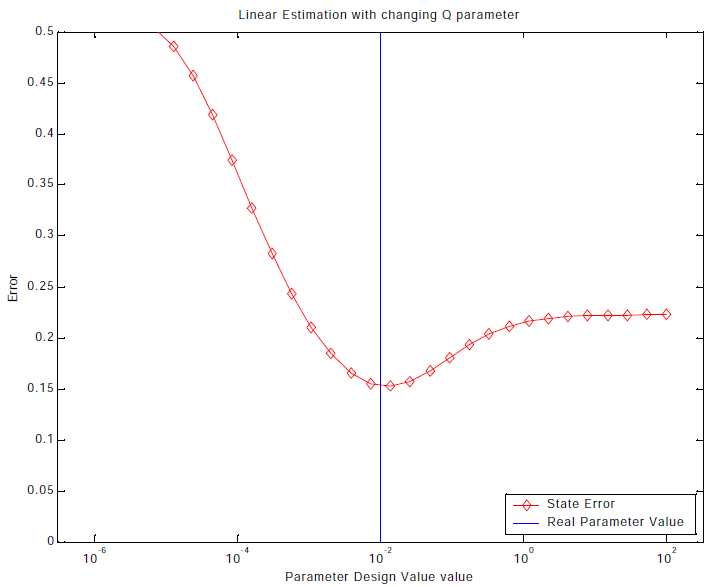
\includegraphics[width=.7\textwidth]{images/adaptiveSensitivity}
\end{figure}
\end{frame}

\begin{frame}{Training KF Parameters}
\begin{itemize}
\item Idea is to log data, including ground truth, and replay through KF while adjusting $Q$ and $R$ to find best estimate compared to ground truth.
\item Use $Q$ and $R$ that generate the minimum error between estimate and ground truth.
\item One error metric minimizes only state errors, other minimizes combination of state errors and covariance.
\end{itemize}
\begin{align*}
\left<R_{\text{res}},Q_{\text{res}}\right> &= \argmin_{R,Q}\sum_{t=0}^T (y_t-h(\mu_t))^TP^{-1}(y_t-h(\mu_t)) \\
\left<R_{\text{pred}},Q_{\text{pred}}\right> &= \argmax_{R,Q}\sum_{t=0}^T -\log|2\pi\Omega_t| \\
&\qquad - (y_t-h(\mu_t))^T\Omega_t^{-1}(y_t-h(\mu_t)) \\
\Omega &= H_t\Sigma_tH_t^T+P
\end{align*}
\end{frame}

\begin{frame}{Kalman Filter Results}
\begin{itemize}
\item Metrics for comparing Kalman filter performance after several stages of changes.
\end{itemize}
% Note for data sources: baseline is 20010107_1037, fixes is 20100107_1411, hand tuned is 20100107_1415, trained is 20100107_1905.
\begin{table}[ht!]
\small
\centering
\begin{tabular}{@{}lllr@{}} \toprule
Stage      & RMS Error (m)  & Return Error (\%) & Distance Traveled (m) \\ \midrule
Baseline   & 10.62          & 1.51              & 224.22 \\
Fix Bugs   & 4.38           & 0.79              & 182.70 \\
Hand Tuned & 4.87           & 1.32              & 184.09 \\
Trained    & 3.64           & 0.99              & 332.62 \\ \bottomrule
\end{tabular}
\label{tab:resultsKF}
\end{table}
\end{frame}

\begin{frame}{Model Based Controller}
\begin{itemize}
\item Replaced PID controller with a model based controller.
\item Model based controller uses kinematic model of robot and Lyapunov stability theory.
\item Significant performance improvements were achieved.
\end{itemize}
\end{frame}

\begin{frame}{Lyapunov Stability}
\begin{itemize}
\item The equilibrium point $x=0$ is stable if
\begin{align*}
V(0) &= 0 \\
V(x) &> 0 \in D-\{0\} \\
\dot{V}(x) &\leq 0 \in D-\{0\}
\end{align*}
\item Asymptotic stability if
\begin{align*}
\dot{V}(x) < 0 \in D - \{0\}
\end{align*}
\item The function $V(x)$ is not guaranteed to exist.
\end{itemize}
\end{frame}

\begin{frame}{Errors In Model Based Controller}
\begin{itemize}
\item $e$ is distance error.
\item $\alpha$ is angle from current heading $\psi$ to waypoint $\theta_e$.
\item $\theta$ is angle from $\theta_e$ to desired heading $\theta^\star$.
\end{itemize}
\begin{figure}[ht!]
	\centering
	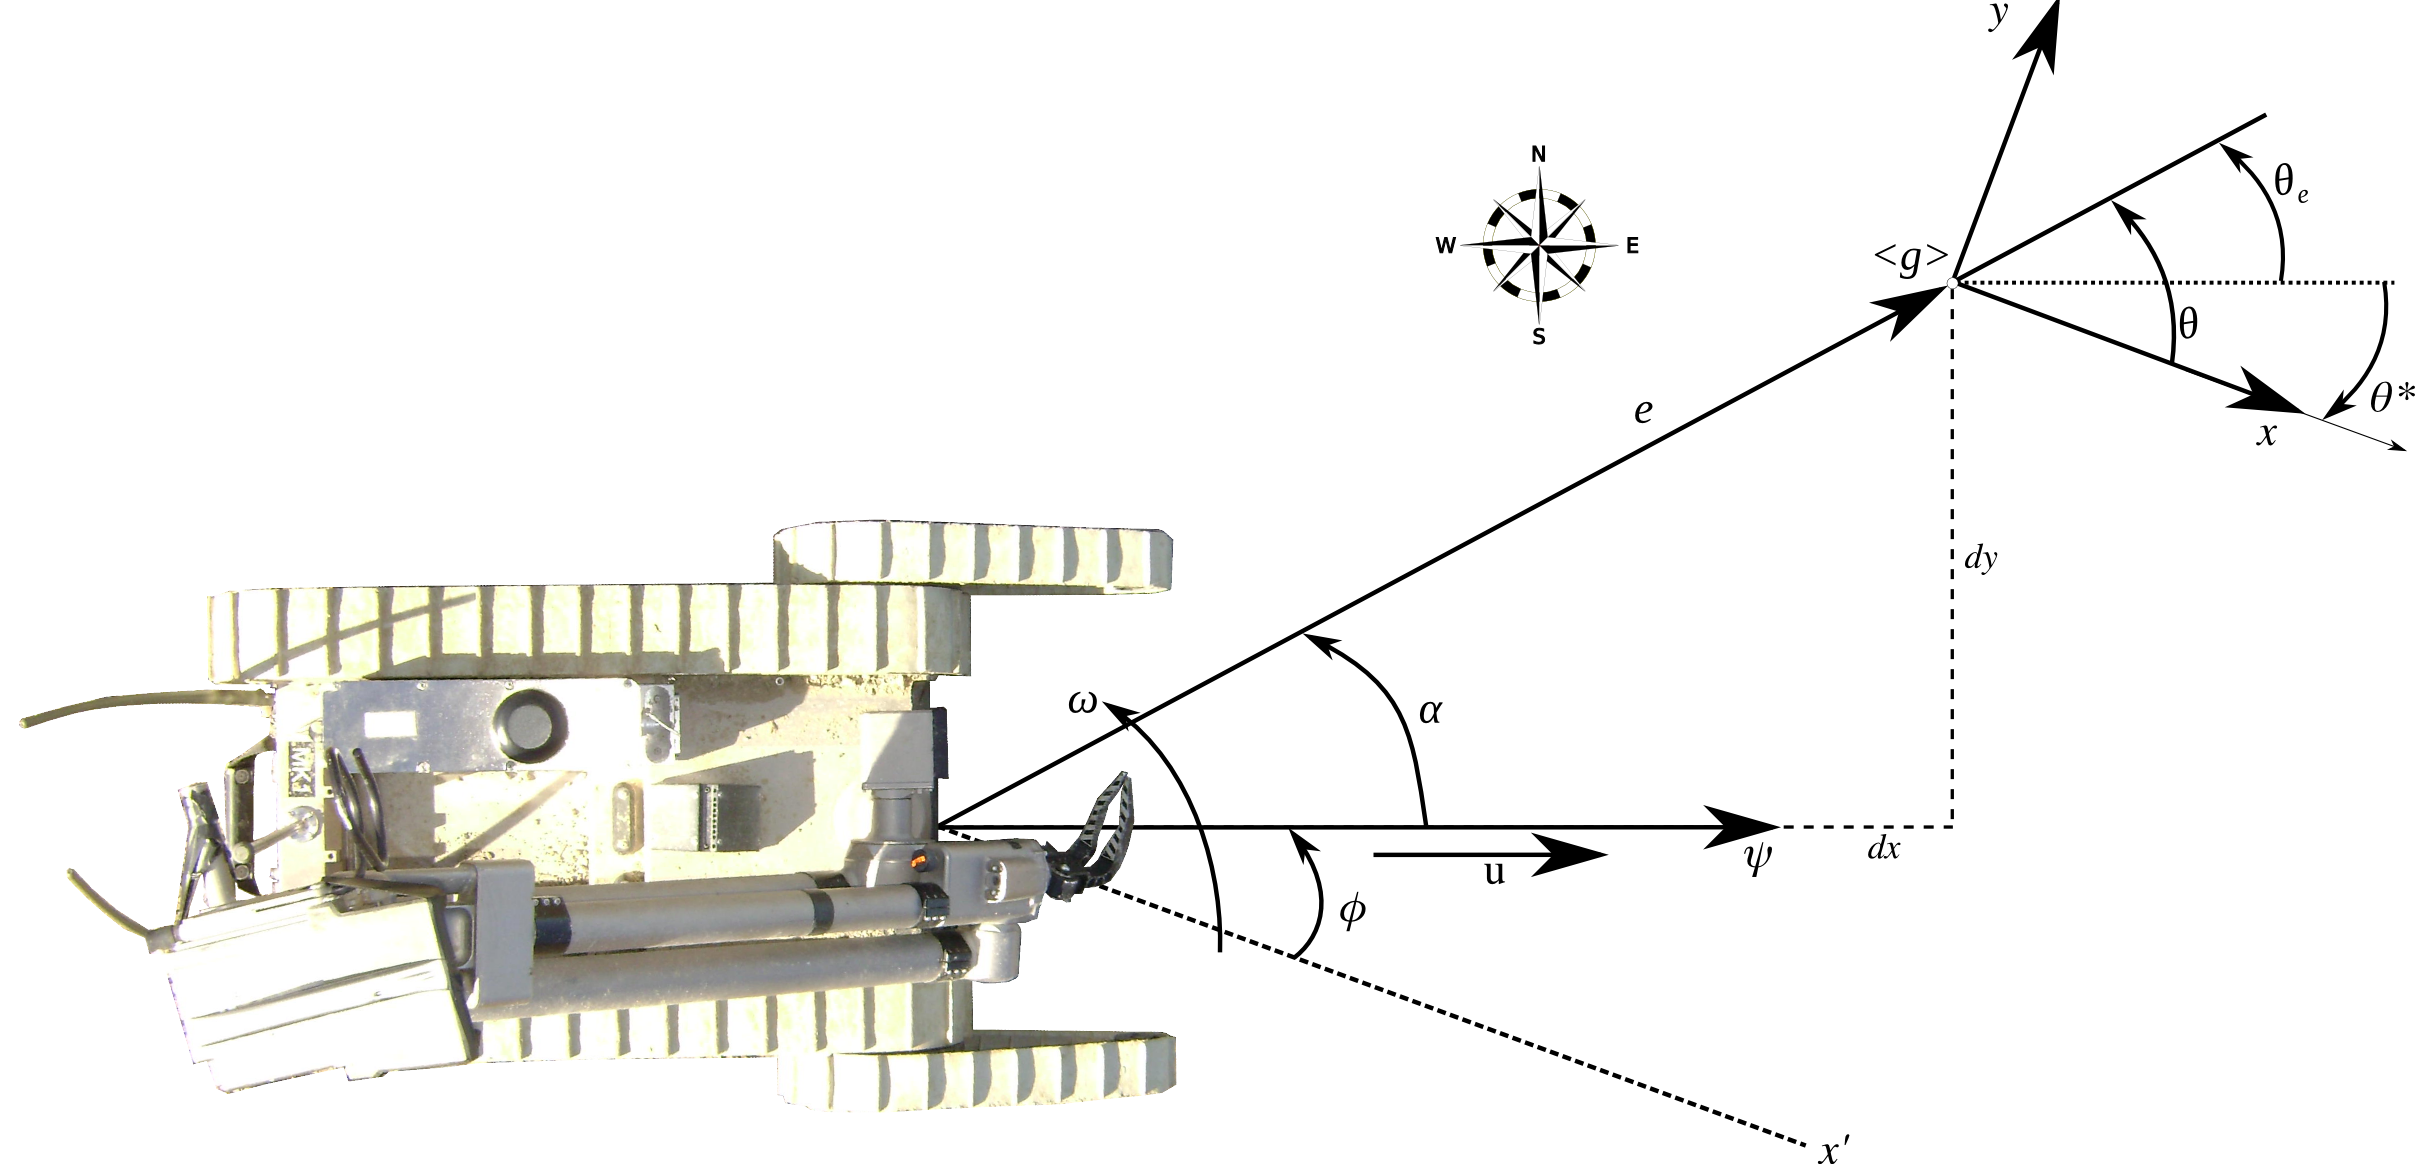
\includegraphics[width=.95\textwidth]{images/packbotlyapunov}
\end{figure}
\end{frame}

\begin{frame}{Control Lyapunov Function}
\begin{itemize}
\item Select a function $V(x) > 0$ and $\dot{V}(x) \leq 0$.
\begin{align*}
V = V_1 + V_2 = \frac{1}{2}\lambda e^2 + \frac{1}{2}\left(\alpha^2+h\theta^2\right)
\end{align*}
\item Robot kinematics model in terms of errors.
\begin{align*}
e &= \sqrt{x^2+y^2} \\
\alpha &= \theta - \phi \\
\theta &= \text{atanh}(y,x)
\end{align*}
\item Error rates from kinematic model.
\begin{align*}
\dot{e} &= -u\cos\alpha \\
\dot{\alpha} &= -\omega + u\frac{\sin\alpha}{e} \\
\dot{\theta} &= u\frac{\sin\alpha}{e}
\end{align*}
\end{itemize}
\end{frame}

\begin{frame}{Control Law}
\begin{itemize}
\item The linear and angular velocity outputs to satisfy asymptotic Lyapunov stability with $V(x)>0$ and $\dot{V}(x) < 0$ are
\begin{align*}
u &= \gamma e\cos\alpha \\
\omega &= k\alpha + \gamma\frac{\cos\alpha\sin\alpha}{\alpha}\left(\alpha+h\theta\right)
\end{align*}
\item Gains are $\gamma$, $h$ and $k$.
\end{itemize}
\end{frame}

\begin{frame}{Moving Target Frame}
\begin{itemize}
\item In many cases it is desirable for robot to maintain speed through intermediate waypoints.
\item When angle errors $\alpha$ and $\theta$ are small want higher speeds.
\item Artificially extended distance error using control Lyapunov function.
\begin{align*}
&\dot{s} =
\begin{cases}
0, & V = \lambda e^2 + (\alpha^2+h\theta^2) > \epsilon \\
f(e,\alpha,\theta), & V = \lambda e^2 + (\alpha^2+h\theta^2) \leq \epsilon
\end{cases} \\
&f(e,\alpha,\theta) = u_{\text{max}} * \text{max}\left(0, 1 - \frac{V}{\epsilon}\right)
\end{align*}
\end{itemize}
\end{frame}

\begin{frame}{Practical Considerations for Gains}
\begin{itemize}
\item If $\alpha < 0.5$ system can be linearized.
\item Linear velocity is proportional to distance error $e$.
\item Angular velocity is proportional to combination of angle errors $\alpha$ and $\theta$.
\item Gain $\gamma$ and eigenvalues of linearized system determine the rate that errors decrease.
\item Eigenvalues based on gains $h$ and $k$.
\item Can deterministically set system response.
\end{itemize}
\end{frame}

\begin{frame}{Setting Gains}
\begin{itemize}
\item For open space environments I used $\gamma=0.25$, $h=1.1$ and $k=2\gamma\sqrt{h}$. This led to
\begin{align*}
\lambda_{\alpha} &= -0.26 \\
\lambda_{\theta} &= -0.26 \\
-\gamma &= -0.25
\end{align*}
\item To keep the robot on straight line segments between waypoints I used $\gamma=0.25$, $h=0.33$ and $k=0.30$ leading to
\begin{align*}
\lambda_{\alpha} &= -0.19 \\
\lambda_{\theta} &= -0.11 \\
-\gamma &= -0.25
\end{align*}
\end{itemize}
\end{frame}

\begin{frame}{Controller Comparison - Long Path Segments}
\begin{table}[ht!]
\small
\centering
\begin{tabular}{@{}llllr@{}} \toprule
Setup & Time (s) & XT (m) & $u_{\text{max}}$ (\%) & Stops \\ \midrule
1     & 82.67    & 0.61   & 33.3                  & 1     \\
2     & 0        & 0      & 0                     & 0     \\
3     & 75.12    & 2.52   & 100.0                 & 3     \\
4     & 71.42    & 2.71   & 100.0                 & 4     \\
5     & 110.09   & 2.42   & 100.0                 & 14    \\
6     & 75.45    & 2.80   & 100.0                 & 5     \\ \bottomrule
\end{tabular}
\end{table}
\end{frame}

\begin{frame}{Controller Comparison - Short Path Segments}
\begin{table}[ht!]
\small
\centering
\begin{tabular}{@{}llllr@{}} \toprule
Setup & Time (s) & XT (m) & $u_{\text{max}}$ (\%) & Stops \\ \midrule
1     & N/A      & N/A    & N/A                   & N/A   \\
2     & 0        & 0      & 0                     & 0     \\
3     & 134.92   & 0.85   & 42.52                 & 20    \\
4     & 75.92    & 0.94   & 50.86                 & 21    \\
5     & 232.09   & 0.79   & 27.90                 & 31    \\
6     & 75.99    & 0.91   & 49.96                 & 23    \\ \bottomrule
\end{tabular}
\end{table}
\end{frame}

\begin{frame}{Controller Comparison - Mixed Path Segments}
\begin{table}[ht!]
\small
\centering
\begin{tabular}{@{}llllr@{}} \toprule
Setup & Time (s) & XT (m) & $u_{\text{max}}$ (\%) & Stops \\ \midrule
1     & N/A      & N/A    & N/A                   & N/A   \\
2     & 0        & 0      & 0                     & 0     \\
3     & 103.39   & 2.51   & 100.0                 & 11    \\
4     & 76.91    & 2.98   & 100.0                 & 12    \\
5     & 164.65   & 2.34   & 100.0                 & 22    \\
6     & 83.84    & 2.87   & 100.0                 & 12    \\ \bottomrule
\end{tabular}
\end{table}
\end{frame}

\begin{frame}{Controller Comparison}
\begin{itemize}
\item Quantitatively there is a trade off between the time to finish a route and the amount of cross track error.
\item Qualitatively it is more reassuring when the robots drive on a straight line between waypoints.
\item Setting $\theta^\star$ as the angle from the previous waypoint to the current waypoint is the recommended setup.
\end{itemize}
\end{frame}

\begin{frame}{Results}
% Put a movie here of the Packbot driving a route.
\begin{itemize}
\item Packbot movie here.
\end{itemize}
\end{frame}

\begin{frame}{Multiple Roots}
% Put a movie here of the Chaos driving a route.
\begin{itemize}
\item Chaos movie here.
\end{itemize}
\end{frame}

\begin{frame}[allowframebreaks]{References}
\nocite{Sights06}
\nocite{Kelly_1994_338}
\nocite{Simon06OptimalEstimation}
\nocite{Mehra72}
\nocite{Abbeel-RSS-05}
\nocite{SakaiKuroda10}
\nocite{MicaelliLyapunov93}
\nocite{Aicardi94}
\nocite{Aicardi_UnicycleLyapunov95}
\nocite{Rusu05RobotuxLyapunov}
\nocite{Gulati08}
\nocite{KimLyapunov05}
\nocite{Lapierre06}
\nocite{Lapierre07}
\nocite{NuchterLyapunov07}
\bibliographystyle{plain}
\bibliography{mybib}
\end{frame}

\end{document}
